\chapter{Left-Corner Parsing}
\label{cha:LeftCorner}

Top-down parsers and bottom-up parsers each turned out to have their advantages as well as their disadvantages.
Top-down parsers are purely predictive.
The input string is only checked against fully built branches --- those that end in a terminal symbol --- but does not guide the prediction process itself.
Bottom-up parsers are purely driven by the input string and lack any kind of predictiveness.
In particular, a bottom-up parser may entertain analyses for the substring spanning from position $i$ to $j$ that are incompatible with the analysis for the substring from $0$ to $i-1$.
Neither behavior seems to be followed by the human parser all the time.

Merely local syntactic coherence effects suggest that the human parser sometimes entertains incompatible parses, just like bottom-up parsers.
But these effects are very rare and very minor compared to, say, the obvious difficulties with garden path sentences.
The human parser is also predictive since ungrammatical sentences are recognized as such as soon as the structure becomes unsalvageable.
At the same time, though, the prediction process differs (at least naively) from pure top-down parsing as it seems to be actively guided by the input.
What we should look at, then, is a formal parsing model that integrates top-down prediction and bottom-up reduction.
Left-corner parsing does exactly that.

\section{Intuition}
\label{sec:LeftCorner_Intuition}

The ingenious idea of left-corner (LC) parsing is to restrict the top-down prediction step such that the parser conjectures $X$ only if there is already some bottom-up evidence for the existence of $X$.
More precisely, the parser conjectures an XP only if a \emph{possible left corner of $X$} has already been identified.
The \emph{left corner of a rewrite rule} is the leftmost symbol on the righthand side of the rewrite arrow. 
For instance, the left corner of NP \rewrite\ Det N is Det.
Thus $Y$ is a possible left corner of $X$ only if the grammar contains a rewrite rule $X$ \rewrite\ $Y$ $\gamma$.
In this case, the parser may conjecture the existence of $X$ and $\gamma$ once it has reached $Y$ in a bottom-up fashion.

Consider our familiar toy grammar.
%
\begin{center}
    \begin{tabular}{rrcl@{\hspace{2em}}rrcl}
        1)  & S   & \rewrite\ & NP VP
        &
        6)  & Det & \rewrite\ & a | the
        \\
        2)  & NP  & \rewrite\ & PN
        &
        7)  & N   & \rewrite\ & car | truck | anvil
        \\
        3)  & NP  & \rewrite\ & Det N
        &
        8)  & PN  & \rewrite\ & Bugs | Daffy
        \\
        4)  & VP  & \rewrite\ & Vi
        &
        9)  & Vi  & \rewrite\ & fell over
        \\
        5)  & VP  & \rewrite\ & Vt NP
        &
        10) & Vt  & \rewrite\ & hit
        \\
    \end{tabular}
\end{center}
%
Rather than conjecturing S \rewrite\ NP VP right away, an LC parser waits until it has identified an NP before it tries to build an S\@.
The NP, in turn, must be found in a bottom-up fashion.
This may involve a sequence of bottom-up reductions: read \emph{Daffy}, reduce \emph{Daffy} to PN, reduce PN to NP\@.
%
\begin{center}
    \begin{tikzpicture}
        \node (Daffy) {Daffy};

        \node [right=3em of Daffy] (PN-Daffy) {Daffy};
        \node [above=1.5em of PN-Daffy] (PN) {PN};

        \node [right=3em of PN-Daffy] (NP-Daffy) {Daffy};
        \node [above=1.5em of NP-Daffy] (NP-PN) {PN};
        \node [above=1.5em of NP-PN]    (NP) {NP};

        \foreach \Source/\Target in {PN-Daffy/PN, NP-Daffy/NP-PN, NP-PN/NP}
            \draw (\Source.north) to (\Target.south);
    \end{tikzpicture}
\end{center}
%
Alternatively, it may involve a mixture of bottom-up reduction and left-corner condition prediction: read \emph{the}, reduce to Det, use the rewrite rule NP \rewrite\ Det N in your top-down prediction, read \emph{anvil}, reduce to N, reduce Det N to NP\@.
%
\begin{center}
    \begin{tikzpicture}
        \node (the) {the};

        \node [right=3em of the] (Det-the) {the};
        \node [above=1.5em of Det-the] (Det) {Det};

        \node [right=3em of Det-the] (NP-the) {the};
        \node [above=1.5em of NP-the] (NP-Det) {Det};
        \node [right=1.5em of NP-Det] (NP-N) {N};
        \node (NP) at ($(NP-Det) !.5! (NP-N)$) [yshift=2.5em] {NP};

        \node [right=5.5em of NP-the] (anvil-the) {the};
        \node [above=1.5em of anvil-the] (anvil-Det) {Det};
        \node [right=1.5em of anvil-Det] (anvil-N) {N};
        \node (anvil-NP) at ($(anvil-Det) !.5! (anvil-N)$) [yshift=2.5em] {NP};
        \node [below=1.5em of anvil-N] (anvil) {anvil};

        \node [right=5.5em of anvil-the] (full-the) {the};
        \node [above=1.5em of full-the] (full-Det) {Det};
        \node [right=1.5em of full-Det] (full-N) {N};
        \node (full-NP) at ($(full-Det) !.5! (full-N)$) [yshift=2.5em] {NP};
        \node [below=1.5em of full-N] (full-anvil) {anvil};

        \foreach \Source/\Target in {%
                                     Det-the/Det,
                                     NP-the/NP-Det,
                                     NP-Det/NP,
                                     NP-N/NP,
                                     anvil-the/anvil-Det,
                                     anvil-N/anvil-NP,
                                     anvil-Det/anvil-NP,
                                     full-the/full-Det,
                                     full-anvil/full-N,
                                     full-Det/full-NP,
                                     full-N/full-NP%
                                 }
            \draw (\Source.north) to (\Target.south);
    \end{tikzpicture}
\end{center}
%
Once the NP has been identified, the parser may use S \rewrite\ NP VP in a prediction step.
The full parse for \emph{the anvil hit Daffy} is depicted in tabular format below.
%
\begin{center}
    \begin{tabular}{r|c|l}
        \textbf{string} & \textbf{rule}          & \textbf{predictions}\\
        the             & read input             & \\
        Det             & Det \rewrite\ the      & \\
                        & left-corner prediction & N to yield NP\\
        anvil           & read input             & N to yield NP\\
        N               & N \rewrite\ anvil      & N to yield NP\\
        NP              & complete prediction    & VP to yield S\\
        hit             & read input             & VP to yield S\\
        Vt              & Vt \rewrite\ hit       & VP to yield S\\
                        & left-corner prediction & VP to yield S, NP to yield VP\\
        Daffy           & read input             & VP to yield S, NP to yield VP\\
        PN              & PN \rewrite\ Daffy     & VP to yield S, NP to yield VP\\
        NP              & NP \rewrite\ PN        & VP to yield S, NP to yield VP\\
        VP              & complete prediction    & VP to yield S\\
        S               & complete prediction    & 
    \end{tabular}
\end{center}

The usual four way split between depth-first or breadth-first on the one hand and left-to-right versus right-to-left on the other makes little sense for left-corner parsers.
The standard LC parser is depth-first left-to-right.
A breadth-first LC parser behaves like a bottom-up parser if LC predictions are delayed, or like a depth-first LC parser if they apply as usual.
And a right-to-left depth-first LC parser has no use for LC predictions since the predicted material has already been inferred in a bottom-up fashion anyways.
%
\begin{center}
    \begin{tikzpicture}
        \Tree
            [.\Lab{S}{6}{12}
                [.\Lab{NP}{3}{5}
                    [.\Lab{Det}{2}{3}
                        \Lab{the}{1}{2}
                    ]
                    [.\Lab{N}{3}{5}
                        \Lab{anvil}{4}{5}
                    ]
                ]
                [.\Lab{VP}{6}{12}
                    [.\Lab{Vt}{8}{9}
                        \Lab{hit}{7}{8}
                    ]
                    [.\Lab{NP}{9}{12}
                        [.\Lab{PN}{11}{12}
                            \Lab{Daffy}{10}{11}
                        ]
                    ]
                ]
            ]
    \end{tikzpicture}
\end{center}

\begin{exercise}
    The tree above shows how LC parsing can be represented via our usual annotation scheme of indices and outdices.
    What would the annotated trees look like for
    %
    \begin{itemize}
        \item a left-to-right breadth-first left-corner parser where
            \begin{itemize}
                \item reading a word can immediately be followed by a single reduction step,
                \item reducing $X$ to $Y$ cannot be immediately followed by a left-corner prediction using $Y$.
            \end{itemize}
        \item a left-to-right breadth-first left-corner parser where
            \begin{itemize}
                \item reading a word can be immediately followed by a single reduction step,
                \item reducing $X$ to $Y$ is immediately followed by a left-corner prediction using $Y$.
            \end{itemize}
        \item a right-to-left depth-first left-corner parser.
    \end{itemize}
\end{exercise}

\begin{exercise}
    Building on your insights from the previous exercise, explain why a breadth-first LC parser is either a bottom-up parser or behaves exactly like a depth-first left-corner parser.
\end{exercise}

\section{Formal Specification}
\label{sec:LeftCorner_Formal}

\subsection{Standard Left-Corner Parser}
\label{sub:LeftCorner_Standard}

Since the usual parameters make little sense for a left-corner parser, we immediately define the parsing schema with some of the control structure incorporated via the familiar dot $\psep$.
The parser has to keep track of four distinct pieces of information:
%
\begin{itemize}
    \item the current position in the string,
    \item any identified nodes $l_i$ that have not been used up by any inference rules yet,
    \item which phrases $p_1, \ldots, p_n$ need to be built according to the left-corner prediction using some $l_i$, and
    \item which phrase is built from $l_i, p_i, \ldots, p_n$
\end{itemize}
%
Our items take the form $[i, \alpha \psep \beta]$, where
%
\begin{itemize}
    \item $i$ is the current position in the string,
    \item $\alpha$ is the list of identified unused nodes (derived via bottom-up reduction), and
    \item $\beta$ is a list of labeled lists of phrases to be built (the top-down predictions).
\end{itemize}
%
For instance, the item [1, \psep [\tsb{NP} N]] encodes that if position 1 is followed by an N, we can build an NP\@.

The parser has a single axiom $[0,\psep]$, and its goal is $[n, S \psep]$.
So the parser has to move from the initial to the last position of the string and end up identifying S\@.
The parser uses five rules, four of which are generalizations of the familiar top-down and bottom-up rules.

\begin{prooftree}
    \AxiomC{$[i, \alpha \psep \beta]$}
    \LeftLabel{\textbf{Shift}\qquad}
    \RightLabel{$a = w_{i}$}
    \UnaryInfC{$[i+1, \alpha a \psep \beta]$}
\end{prooftree}

\begin{prooftree}
    \AxiomC{$[i, \alpha \gamma \psep \beta]$}
    \LeftLabel{\textbf{Reduce}\qquad}
    \RightLabel{$N \rewrite \gamma \in R$}
    \UnaryInfC{$[i, \alpha N \psep \beta]$}
\end{prooftree}

\begin{prooftree}
    \AxiomC{$[i, \alpha N \psep [_M\ N \gamma ]\ \beta]$}
    \LeftLabel{\textbf{Scan}\qquad}
    \UnaryInfC{$[i, \alpha \psep [_M\ \gamma ]\ \beta]$}
\end{prooftree}

\begin{prooftree}
    \AxiomC{$[i, \alpha N \psep \beta]$}
    \LeftLabel{\textbf{Predict}\qquad}
    \RightLabel{$M \rewrite N \gamma \in R$}
    \UnaryInfC{$[i, \alpha \psep [_M\ \gamma ]\ \beta]$}
\end{prooftree}

\begin{prooftree}
    \AxiomC{$[i, \alpha \psep [_M\ ]\ \beta]$}
    \LeftLabel{\textbf{Complete}\qquad}
    \UnaryInfC{$[i, \alpha M \psep \beta]$}
\end{prooftree}

The shift rule reads in new input, and the reduce rule replaces the right-hand side of a rewrite rule by its left-hand side, thereby building structure in the usual bottom-up fashion.
The scan rule eliminates a predicted symbol against an existing one, just like the top-down scan rule eliminates a predicted terminal symbol if a matching symbol can be found in the input at this position.%

The predict rule necessarily extends the prediction mechanism of a standard top-down parser since left-corner prediction is conditioned both bottom-up, when it infers the symbol to the left of the rewrite arrow, and top-down, when it infers the sister nodes to the right.
An existing left-corner $N$ is removed, and instead we add to $\beta$ a list that is labeled with the conjectured mother of $N$ and contains the conjectured sisters of $N$.
The completion rule, finally, states that once we have completely exhausted a list --- i.e.\ all the conjectured siblings have been identified --- the phrase that can be built from the elements in this list is promoted from a mere conjecture to a certainty, which is formally encoded by pushing it to the left side of $\psep$.

\begin{examplebox}[Left-corner parse of \emph{The anvil hit Daffy}]
    \label{ex:LC_ParseTable}
    \phantom{a}
    \begin{center}
        \begin{tabular}{r|l}
            \textbf{parse item} & \textbf{inference rule}\\
            $\lbrack$0,\psep,]              & axiom\\
            $\lbrack$1,the \psep,]          & shift\\
            $\lbrack$1,Det \psep,]          & reduce(6)\\
            $\lbrack$1,\psep [\tsb{NP} N]]       & predict(3)\\
            $\lbrack$2,anvil \psep [\tsb{NP} N]] & shift\\
            $\lbrack$2,N \psep [\tsb{NP} N]] & reduce(7)\\
            $\lbrack$2,\psep [\tsb{NP}]] & scan\\
            $\lbrack$2,NP \psep ] & complete\\
            $\lbrack$2,\psep [\tsb{S} VP]] & predict(1)\\
            $\lbrack$3,hit \psep [\tsb{S} VP]] & shift\\
            $\lbrack$3,Vt \psep [\tsb{S} VP]] & reduce(10)\\
            $\lbrack$3,\psep [\tsb{VP} NP] [\tsb{S} VP]] & predict(5)\\
            $\lbrack$4,Daffy \psep [\tsb{VP} NP] [\tsb{S} VP]] & shift\\
            $\lbrack$4,PN \psep [\tsb{VP} NP] [\tsb{S} VP]] & reduce(8)\\
            $\lbrack$4,NP \psep [\tsb{VP} NP] [\tsb{S} VP]] & reduce(2)\\
            $\lbrack$4,\psep [\tsb{VP}] [\tsb{S} VP]] & scan\\
            $\lbrack$4, VP \psep [\tsb{S} VP]] & complete\\
            $\lbrack$4,\psep [\tsb{S}]] & scan\\
            $\lbrack$4,S \psep] & complete\\
        \end{tabular}
    \end{center}
\end{examplebox}
%
\begin{exercise}
    Consider the minimally different \emph{The anvil suddenly hit Daffy} and \emph{The anvil hit Daffy suddenly}.    
    \begin{enumerate}
        \item Add appropriate rewrite rules to our toy grammar so that they can generate these sentences, with \emph{suddenly} analyzed as a VP-adjunct.
        \item Write down the parse tables for both sentences.
        \item At what point do they differ from the one for \emph{The anvil hit Daffy}?
        \item Upon careful inspection, it is clear that \emph{The anvil suddenly hit Daffy} is less likely to be misanalyzed by the LC parser than \emph{The anvil hit Daffy suddenly}.
            Explain why!
    \end{enumerate}
\end{exercise}

The choice of $\psep$ as a separator with identified material to the left and predicted material to the right is not accidental.
Recall that the recursive descent parser is a purely predictive parser, and in all its parse items $\psep$ occurred to the very left.
So the predicted material was trivially to the right of $\psep$.
Similarly, the shift reduce parser is completely free of any predictions, and the material built via shift and reduce was always to the left of $\psep$.
So $\psep$ indicates the demarkation line between confirmed and conjectured material in all three parsers.
Viewed from this perspective, the inference rules of the left-corner parser highlight its connections to top-down and bottom-up parsing.
This becomes even more apparent when the inference rules of the parser are aligned next to each other as in Tab.~\ref{tab:LeftCorner_ParserComparison}) (the empty sides of recursive descent and shift reduce parsers are filled by variables to highlight the parallel to LC parsing).
%
\begin{table}[tbph]
    \begin{tabular}{rp{2em}ccc}
             & & \textbf{Top-Down}
             & \textbf{Bottom-Up}
             & \textbf{Left-Corner}\\[1em]
             \hline
             \\[1em]
        \textbf{Axiom} & &
            \(
                [0,\psep S]
            \)
            &
            \(
                [,0]
            \)
            &
            \(
                [0,\psep]
            \)
            \\[2em]
        \textbf{Goal} & &
            \(
                [n,\psep]
            \)
            &
            \(
                [S\psep,n]
            \)
            &
            \(
                [n,S \psep]
            \)
            \\[2em]
        \textbf{Scan} & &
            \(
                \dfrac{[i, \alpha \psep a \beta]}%
                    {[i+1, \alpha \psep \beta]}
            \)
            &
            &
            \(
                \dfrac{[i, \alpha N \psep [_M\ N \gamma ]\ \beta]}%
                    {[i, \alpha \psep [_M\ \gamma ]\ \beta]}
            \)
            \\[2em]
        \textbf{Shift} & &
            &
            \(
                \dfrac{[\alpha \psep \beta, j]}%
                    {[\alpha a \psep \beta, j+1]}
            \)
            &
            \(
                \dfrac{[i, \alpha \psep \beta]}%
                    {[i+1, \alpha a \psep \beta]}
            \)
            \\[2em]
        \textbf{Predict} & &
            \(
                \dfrac{[i, \alpha \psep N \beta]}%
                    {[i, \alpha \psep \gamma \beta]}
            \)
            &
            &
            \(
                \dfrac{[i, \alpha N \psep \beta ]}%
                    {[i, \alpha \psep [_M\ \gamma ]\ \beta ]}
            \)
            \\[2em]
        \textbf{Reduce} & &
            &
            \(
                \dfrac{[\alpha \gamma \psep \beta, j]}%
                    {[\alpha N \psep \beta, j]}
            \)
            &
            \(
                \dfrac{[i, \alpha \gamma \psep \beta]}%
                    {[i, \alpha N \psep \beta]}
            \)
            \\[2em]
        \textbf{Complete} & &
            &
            & 
            \(
                \dfrac{[i, \alpha \psep [_M\ ]\ \beta]}%
                    {[i, \alpha M \psep \beta ]}
            \)
    \end{tabular}
\caption{Comparison of recursive descent, shift reduce, and left-corner parser}
\label{tab:LeftCorner_ParserComparison}
\end{table}

The connections between the parsers can be strengthened even more.
The scan rule of the recursive descent parser does not quite match the one in the LC parser, it looks as if the two are performing very different tasks.
The former checks a prediction against the input, the latter cancels out a prediction against some previously found material.
But this is in fact just a generalization of recursive descent scanning from terminals to non-terminals.
To make this more apparent, we can decompose the recursive descent scanning rule into a shift rule and a second rule that closely mirrors the LC scan rule:
%
\begin{prooftree}
    \AxiomC{$[i, \psep \beta]$}
    \LeftLabel{\textbf{Shift}\qquad}
    \RightLabel{$a = w_{i}$}
    \UnaryInfC{$[i+1, a \psep \beta]$}
\end{prooftree}
%
\begin{prooftree}
    \AxiomC{$[i, a \psep a \beta]$}
    \LeftLabel{\textbf{Scan}\qquad}
    \UnaryInfC{$[i,\psep \beta]$}
\end{prooftree}
%
So the scan rule we used for the recursive descent parser is just a convenient shorthand for shift followed by scan as defined above.
This is also called a \emph{step contraction} \citep{Sikkel97}: a sequence of inference rules is compressed into the application of a single inference rule.

\begin{exercise}
    The LC parser itself also contains a step contraction.
    Show that the reduce rule is just a step contraction of two other inference rules.
\end{exercise}

\subsection{Adding Top-Down Filtering}
As the predict rule of the LC parser is conditioned by the presence of recognized material, bottom-up information serves to prune down the number of possible predictions.
Note, however, that reduction steps can still apply very freely.
This is somewhat wasteful.
Top-down information should also be used to restrict the set of reductions, and as we will see next this is very simple in an LC parser.

Consider once again the LC parse for the sentence \emph{the anvil hit Daffy}, and suppose that our grammar allows for \emph{hit} to be reduced to either N or Vt (only the latter is the case in our usual toy grammar).
The parser does not encounter \emph{hit} in the input until a VP has already been predicted: first the parser recognizes then NP, then it uses NP as the left corner for predicting S and VP, and then it shifts one word to the right in the input and finally reads in \emph{hit}.
A quick glance at our grammar will reveal that it is impossible for \emph{hit} to be a noun in this parse.
Obviously \emph{hit} must be the leftmost word of the string spanned by the VP, and there is no sequence of rewrite rules in our grammar that could generate a VP with a noun at its left edge.
If we could incorporate that line of reasoning into the inference rules of the parser, we might be able to save us a lot of work exploring doomed parses.

This idea can be made precise by generalizing the notion of left corner.
So far, a left corner was defined as the leftmost element of the right-hand side of a rule.
This will now be given the more specific term \emph{direct left corner}, and $X$ is a left corner of $Z$ iff $X = Z$ or there are $Y_1, \ldots, Y_n$ such that $X$ is the left corner of $Y_1$, each $Y_i$ is a left corner of $Y_{i+1}$, and $Y_n$ is the left corner of $Y_n$.
More succinctly:
%
\begin{definition}[Left Corner]
    The \emph{direct left corner relation} holds between $X$ and $Y$ in grammar $G$ iff $G$ contains a rewrite rule $Y \rewrite X \beta$, $\beta \in (N \cup T)^*$.
    The \emph{left corner relation} $\LeftCorner$ is the reflexive transitive closure of the direct left corner relation.
    We write $\LeftCorner(Y)$ for the set $\setof{X \mid \tuple{X,Y} \in \LeftCorner}$ of left corners of $Y$.
\end{definition}
%
If this is still confusing to you, just remember that $X$ is a left corner of $Y$ iff our grammar can generate a subtree with root $Y$ where $X$ is the root or occurs along the leftmost branch.

Keep in mind that we can compute in advance for every pair of non-terminals $X$ and $Y$ whether $X$ is a left corner of $Y$.
So we can use the left corner relation as a side condition in our inference rules without worrying about whether they can still be refined into a parsing system.
%
\begin{exercise}
    Explain step by step why this is the case.
    What properties of CFGs, parsing systems, and the left corner relation are relevant here?
\end{exercise}
%
All we have to do now is to add a side condition to the reduce rule that implements top-down filtering.
%
\begin{prooftree}
    \AxiomC{$[i, \alpha \gamma \psep \beta]$}
    \LeftLabel{\textbf{Reduce}\qquad}
    \RightLabel{$N \rewrite \gamma \in R$, and if $\beta = [_X Y] \delta$ then $N \in \LeftCorner(Y)$}
    \UnaryInfC{$[i, \alpha N \psep \beta]$}
\end{prooftree}
%
\begin{exercise}
    Consider a modified version of our toy grammar that also contains the rewrite rule N \rewrite\ hit.
    For each non-terminal, compute its set of left corners.
    Then write down a detailed parse table of \emph{the anvil hit Daffy} and highlight the step at which the parser is forced to reduce \emph{hit} to a verb.
\end{exercise}
%
\begin{exercise}
    In an earlier exercise you had to show that the reduce rule is a step contraction of two other rules.
    Consequently, restricting the applicability of reduce is not enough to add top-down filtering since the parser also has an alternative means of reducing that is still completely unrestricted.
    Try to patch up this loop hole.
    \emph{Hint}: you can either put a similar restriction on those other two rules or ensure that the two can no longer be used as an alternative to reduce.
\end{exercise}


\subsection{Generalized Left-Corner Parsing}
\label{sub:LeftCorner_Generalized}

The left-corner parser combines top-down and bottom-up in a specific manner: one symbol needs to be found bottom-up before a top-down prediction can take place.
This weighting of bottom-up and top-down can be altered by changing the number of symbols that need to be present.
That is to say, the left-corner of a rule is no longer just the leftmost symbol of its right side, but rather a prefix of the right side.
For instance, if the number is increased to $2$, then NP \rewrite\ Det A N could be used to predict N and NP only after Det and A have been identified.
We can also let this threshold vary between rewrite rules to hold off on cases with more ambiguity while committing quickly whenever a specific rewrite step is much more likely than the alternatives.

An LC parser where the threshold for predictions is allowed to vary for each rule is called a \emph{generalized left-corner parser} (GLC).
It uses the same rules as a standard left-corner parser, except that the prediction rule is slightly modified.
First, assume that each rewrite rule is associated with a specific index that indicates the threshold at which the left corner prediction is triggered.
We can indicate this position pictorially by putting a $\star$ at the appropriate position in the rewrite rule.
For example, NP \rewrite\ Det A N might be written NP \rewrite Det A $\star$ N.
Then we can generalize the predict rule from a simple LC parser to a GLC parser.
%
\begin{prooftree}
    \AxiomC{$[i, \alpha \delta \psep \beta]$}
    \LeftLabel{\textbf{Predict}\qquad}
    \RightLabel{$M \rewrite \delta \star \gamma \in R$}
    \UnaryInfC{$[i, \alpha \psep [_M\ \gamma ]\ \beta]$}
\end{prooftree}

The GLC parser points out yet another close connection to top-down and bottom-up parsing, which now turn out to simply be special cases of the latter.
A bottom-up parser is a GLC parser where the star is always at the end of a rewrite rule, so $M$ is predicted only if all its daughters have already been identified.
In this case the prediction rule turns $[i, \alpha \delta \psep \beta]$ into $[i, \alpha \psep [_M] \beta]$, which the completion rule turns into $[i, \alpha M \psep]$.
So bottom-up reduction is a step contraction of prediction followed by completion.

A top-down parser is similar to a GLC parser where the star is always at the beginning of the right-hand side of the rewrite rule, so the prediction rule is never restricted by a left corner.
This analogy is not completely right, however, because such a GLC parser can predict any rule at any given point, whereas the top-down parser must make predictions that are licit rewritings of non-terminal symbols in the parse items.
But LC parsers are nonetheless very closely related to top-down parsing, as we will see in the next section.

\paragraph{An important terminological remark} The term generalized left-corner parser is used very differently in psycholinguistics and computer science.
The definition above is the psycholinguistic one.
In computer science, there are at least two alternative definitions.
One is simply the standard LC parser covered in this section --- GLC is then used to distinguish it from a so-called deterministic left-corner parser (which is of little interest to us at this point since natural language sentences are ambiguous and thus inherently non-deterministic).
The other usage of GLC refers to an LC parser with a particular graph-based data structure.
% fixme: add references


\section{Left-Corner Parsing as Top-Down Parsing} 
\label{sec:LC_GrammarTransform}
Remember from the discussion in Cha.~\ref{cha:ParserOverview} that parsers can be viewed as algorithms for constructing intersection grammars in an incremental fashion.
From this perspective, a parser is a particular kind of map from grammars to grammars, which is also called a \emph{grammar transform}.
We will now look at another instance of this idea: an LC parser for grammar $G$ is a top-down parser operating on the \emph{left-corner transform} of $G$ \citep{RosenkrantzLewis70,AhoUllman72}.

Intuitively, the left-corner transform rotates trees by 90 degrees to the right so that the bottom left corner becomes the top left corner (cf.\ Fig.~\ref{fig:LC_TransformTreeComparison}).
As a result, left corners end up c-commanding their mother as well as their right siblings.
Thanks to their new structural prominence, left corners are now also conjectured by the top-down parser before the other nodes.
While this may sound rather confusing, the left corner transform is actually very easy to define.
%
\begin{definition}
    Let $G \is \tuple{N, T, S, R}$ be a CFG\@.
    The \emph{left-corner transform} of $G$ is the CFG $G^\LeftCorner \is \tuple{N', T, S, R'}$ such that
    %
    \[
        \begin{array}{ll}
            A \rewrite\ a\ A\mhyphen a               & \text{for all $A \in N$ and $a \in T$}\\
            A \rewrite\ A\mhyphen B                  & \text{for all $A \in N$ and $B \rewrite \emptystring \in R$}\\ A\mhyphen X \rewrite\ \beta\ A\mhyphen B & \text{for all $A \in N$ and $B \rewrite X \beta \in R$}\\
            A\mhyphen A \rewrite \emptystring        & \text{for all $A \in N$}
        \end{array}
    \]
\end{definition}
%
\begin{examplebox}[Left-Corner Transform of our Example Grammar]
    Our toy example grammar consists of 
    \begin{itemize}
        \item the non-terminals S, NP, VP, Det, N, PN, Vi, and Vt,
        \item the terminals a, the, car, truck, anvil, Bugs, Daffy, fell over, hit,
        \item the ten rewrite rules listed below.
    \end{itemize}
    %
    \begin{center}
        \begin{tabular}{rrcl@{\hspace{2em}}rrcl}
            1)  & S   & \rewrite & NP VP
            &
            6)  & Det & \rewrite & a | the
            \\
            2)  & NP  & \rewrite & PN
            &
            7)  & N   & \rewrite & car | truck | anvil
            \\
            3)  & NP  & \rewrite & Det N
            &
            8)  & PN  & \rewrite & Bugs | Daffy
            \\
            4)  & VP  & \rewrite & Vi
            &
            9)  & Vi  & \rewrite & fell over
            \\
            5)  & VP  & \rewrite & Vt NP
            &
            10) & Vt  & \rewrite & hit
            \\
        \end{tabular}
    \end{center}
    %
    We now apply the left-corner transform.
    First we have to add a rule of the form $A \rewrite a A\mhyphen a$ for all $A \in N$ and $a \in T$.
    Even with our small toy grammar that is a lot of rules.
    %
    \begin{center}
        \begin{tabular}{rcl@{\hspace{2em}}rcl}
            S & \rewrite & a S-a
            &
            S & \rewrite & the S-the
            \\
            S & \rewrite & car S-car
            &
            S & \rewrite & truck S-truck
            \\
            S & \rewrite & anvil S-anvil
            &
            S & \rewrite & Bugs S-Bugs
            \\
            S & \rewrite & Daffy S-Daffy
            &
            S & \rewrite & fell\_over S-fell\_over
            \\
            S & \rewrite & hit S-hit
        \end{tabular}

        \begin{tabular}{rcl@{\hspace{2em}}rcl}
            NP & \rewrite & a NP-a
            &
            NP & \rewrite & the NP-the
            \\
            NP & \rewrite & car NP-car
            &
            NP & \rewrite & truck NP-truck
            \\
            NP & \rewrite & anvil NP-anvil
            &
            NP & \rewrite & Bugs NP-Bugs
            \\
            NP & \rewrite & Daffy NP-Daffy
            &
            NP & \rewrite & fell\_over NP-fell\_over
            \\
            NP & \rewrite & hit NP-hit
        \end{tabular}

        \begin{tabular}{rcl@{\hspace{2em}}rcl}
            VP & \rewrite & a VP-a
            &
            VP & \rewrite & the VP-the
            \\
            VP & \rewrite & car VP-car
            &
            VP & \rewrite & truck VP-truck
            \\
            VP & \rewrite & anvil VP-anvil
            &
            VP & \rewrite & Bugs VP-Bugs
            \\
            VP & \rewrite & Daffy VP-Daffy
            &
            VP & \rewrite & fell\_over VP-fell\_over
            \\
            VP & \rewrite & hit VP-hit
        \end{tabular}

        \begin{tabular}{rcl@{\hspace{2em}}rcl}
            Det & \rewrite & a Det-a
            &
            Det & \rewrite & the Det-the
            \\
            Det & \rewrite & car Det-car
            &
            Det & \rewrite & truck Det-truck
            \\
            Det & \rewrite & anvil Det-anvil
            &
            Det & \rewrite & Bugs Det-Bugs
            \\
            Det & \rewrite & Daffy Det-Daffy
            &
            Det & \rewrite & fell\_over Det-fell\_over
            \\
            Det & \rewrite & hit Det-hit
        \end{tabular}

        \begin{tabular}{rcl@{\hspace{2em}}rcl}
            N & \rewrite & a N-a
            &
            N & \rewrite & the N-the
            \\
            N & \rewrite & car N-car
            &
            N & \rewrite & truck N-truck
            \\
            N & \rewrite & anvil N-anvil
            &
            N & \rewrite & Bugs N-Bugs
            \\
            N & \rewrite & Daffy N-Daffy
            &
            N & \rewrite & fell\_over N-fell\_over
            \\
            N & \rewrite & hit N-hit
        \end{tabular}

        \begin{tabular}{rcl@{\hspace{2em}}rcl}
            PN & \rewrite & a PN-a
            &
            PN & \rewrite & the PN-the
            \\
            PN & \rewrite & car PN-car
            &
            PN & \rewrite & truck PN-truck
            \\
            PN & \rewrite & anvil PN-anvil
            &
            PN & \rewrite & Bugs PN-Bugs
            \\
            PN & \rewrite & Daffy PN-Daffy
            &
            PN & \rewrite & fell\_over PN-fell\_over
            \\
            PN & \rewrite & hit PN-hit
        \end{tabular}

        \begin{tabular}{rcl@{\hspace{2em}}rcl}
            Vi & \rewrite & a Vi-a
            &
            Vi & \rewrite & the Vi-the
            \\
            Vi & \rewrite & car Vi-car
            &
            Vi & \rewrite & truck Vi-truck
            \\
            Vi & \rewrite & anvil Vi-anvil
            &
            Vi & \rewrite & Bugs Vi-Bugs
            \\
            Vi & \rewrite & Daffy Vi-Daffy
            &
            Vi & \rewrite & fell\_over Vi-fell\_over
            \\
            Vi & \rewrite & hit Vi-hit
        \end{tabular}

        \begin{tabular}{rcl@{\hspace{2em}}rcl}
            Vt & \rewrite & a Vt-a
            &
            Vt & \rewrite & the Vt-the
            \\
            Vt & \rewrite & car Vt-car
            &
            Vt & \rewrite & truck Vt-truck
            \\
            Vt & \rewrite & anvil Vt-anvil
            &
            Vt & \rewrite & Bugs Vt-Bugs
            \\
            Vt & \rewrite & Daffy Vt-Daffy
            &
            Vt & \rewrite & fell\_over Vt-fell\_over
            \\
            Vt & \rewrite & hit Vt-hit
        \end{tabular}
    \end{center}
    %
    Our grammar contains no rules that rewrite a non-terminal as the empty string, so we can skip the second step of the transform.
    Next we have to add rules of the form $A\mhyphen X \rewrite \beta\ A\mhyphen B$ for all non-terminals $A$ and every $B$ such that $B \rewrite X\ \beta$.
    We only list the rewrite rules for S, but exactly the same rules exist for every other non-terminal.
    %
    \begin{center}
        \begin{tabular}{rcl@{\hspace{2em}}rcl}
            S-NP & \rewrite & VP S-S
            &
            S-a & \rewrite & S-Det
            \\
            S-PN & \rewrite & S-NP
            &
            S-the & \rewrite & S-Det
            \\
            S-Det & \rewrite & N S-NP
            &
            S-car & \rewrite & S-N
            \\
            S-Vi & \rewrite & S-VP
            &
            S-truck & \rewrite & S-N
            \\
            S-Vt & \rewrite & NP S-VP
            &
            S-anvil & \rewrite & S-N
            \\
            & & &
            S-Bugs & \rewrite & S-PN
            \\
            & & &
            S-Daffy & \rewrite & S-PN
            \\
            & & &
            S-fell\_over & \rewrite & S-Vi
            \\
            & & &
            S-hit & \rewrite & S-Vt
        \end{tabular}
    \end{center}
    %
    Finally, we add $A\mhyphen A \rewrite \emptystring$ for all non-terminals $A$ of the original grammar.
    %
    \begin{center}
        \begin{tabular}{rcl@{\hspace{2em}}rcl}
            S-S & \rewrite & \emptystring
            &
            Det-Det & \rewrite & \emptystring
            \\
            NP-NP & \rewrite & \emptystring
            &
            N-N & \rewrite & \emptystring
            \\
            VP-VP & \rewrite & \emptystring
            &
            PN-PN & \rewrite & \emptystring
            \\
            & & &
            Vi-Vi & \rewrite & \emptystring
            \\
            & & &
            Vt-Vt & \rewrite & \emptystring
        \end{tabular}
    \end{center}
    %
    This is an enormous grammar with a confusing arrangements of rules, which is furthermore exacerbated by the unfortunate fact that most of these rules cannot occur in a well-formed derivation.
    Fortunately there are algorithms for pruning away such useless rules \citep[cf.]{GruneJacobs08}.
    %fixme: add page numbers
    The compacted grammar is still much bigger than the original though.
    %
    %fixme: pruned grammar here
    %
\end{examplebox}

Even an extended look at the transformed grammar in the example above does not readily reveal how it relates top-down parsing to LC parsing.
However, things become clearer when one compares which tree the original grammar generates for \emph{The anvil hit Daffy} to the tree licensed by the transformed grammar.
Both trees are shown in Fig.~\ref{fig:LC_TransformTreeComparison}.
%
\begin{figure}[tbph]
\centering
    \begin{tikzpicture}
        \Tree
            [.S
                [.NP
                    [.Det the ]
                    [.N anvil ]
                ]
                [.VP
                    [.Vt hit ]
                    [.NP
                        [.PN
                            Daffy
                        ]
                    ]
                ]
            ]
    \end{tikzpicture}
    %
    \hspace{2em}
    %
    \begin{tikzpicture}[
        level 1/.style = { sibling distance = -4em },
        level 3/.style = { sibling distance = -2em },
        level 5/.style = { sibling distance = -4em }
        ]
        \Tree
            [.S
                the
                [.S-the
                    [.S-Det
                        [.N
                            anvil
                            [.N-anvil
                                [.N-N
                                    $\emptystring$
                                ]
                            ]
                        ]
                        [.S-NP
                            [.VP
                                hit
                                [.VP-hit
                                    [.VP-Vt
                                        [.NP
                                            Daffy
                                            [.NP-Daffy
                                                [.NP-PN
                                                    [.NP-NP
                                                        $\emptystring$
                                                    ]
                                                ]
                                            ]
                                        ]
                                        [.VP-VP
                                            $\emptystring$
                                        ]
                                    ]
                                ]
                            ]
                            [.S-S
                                $\emptystring$
                            ]
                        ]
                    ]
                ]
            ]
    \end{tikzpicture}
\caption{Parse tree for \emph{The anvil hit Daffy} with original and transformed grammar}
\label{fig:LC_TransformTreeComparison}
\end{figure}
%
When the transformed tree is traversed in the fashion of a recursive descent parser, it closely lines up with the LC parse table for \emph{the anvil hit Daffy} in example~\ref{ex:LC_ParseTable}.
Figure~\ref{fig:LC_AnnotatedTransformTree} depicts this in full detail.
%
\begin{figure}[tbph]
\centering
    \begin{tikzpicture}[
        level 1/.style = { sibling distance = -4em },
        level 3/.style = { sibling distance = 2em },
        level 4/.style = { sibling distance = 4em },
        level 5/.style = { sibling distance = -4em }
        ]
        \Tree
            [.\node(0){S};
                \node(00){the};
                [.\node(01){S-the};
                    [.\node(010){S-Det};
                        [.\node(0100){N};
                            \node(01000){anvil};
                            [.\node(01001){N-anvil};
                                [.\node(010010){N-N};
                                    \node(0100100){$\emptystring$};
                                ]
                            ]
                        ]
                        [.\node(0101){S-NP};
                            [.\node(01010){VP};
                                \node(010100){hit};
                                [.\node(010101){VP-hit};
                                    [.\node(0101010){VP-Vt};
                                        [.\node(01010100){NP};
                                            \node(010101000){Daffy};
                                            [.\node(010101001){NP-Daffy};
                                                [.\node(0101010010){NP-PN};
                                                    [.\node(01010100100){NP-NP};
                                                        \node(010101001000){$\emptystring$};
                                                    ]
                                                ]
                                            ]
                                        ]
                                        [.\node(01010101){VP-VP};
                                            \node(010101010){$\emptystring$};
                                        ]
                                    ]
                                ]
                            ]
                            [.\node(01011){S-S};
                                \node(010110){$\emptystring$};
                            ]
                        ]
                    ]
                ]
            ]

        % labels
        \foreach \Node/\Direction/\Label in {%
                                            0/left/axiom,
                                            01/right/shift,
                                            010/right/reduce(6),
                                            0100/left/predict(3),
                                            01001/above right/shift,
                                            010010/left/reduce(7),
                                            0100100/left/scan,
                                            0101/right/complete,
                                            01010/right/predict(1),
                                            010101/right/shift,
                                            0101010/right/reduce(10),
                                            01010100/left/predict(5),
                                            010101001/below left/shift,
                                            0101010010/right/reduce(8),
                                            01010100100/right/reduce(2),
                                            010101001000/right/scan,
                                            01010101/right/complete,
                                            010101010/right/scan,
                                            01011/right/complete
                                            }
            {
            \node (lab-\Node) [\Direction=2em of \Node, text = {blue!75}] {\Label};
            \draw[blue!75,->] (lab-\Node) to (\Node);
            }
    \end{tikzpicture}
\caption{Recursive descent traversal of the parse tree closely mirrors the steps of an LC parser}
\label{fig:LC_AnnotatedTransformTree}
\end{figure}
%
Closer analysis of the tree also reveals that the names of the non-terminals were not chosen arbitrarily.
Instead, they follow a simple pattern were the hyphen serves a similar function as the dot in our items: recognized material is to the right of the hyphen, conjectured material to its left (note that this is the exact reverse of the order used in our parse items).
The node S-NP, for instance, encodes the fact that we are conjecturing an S and have successfully identified its NP subtree.
A non-terminal $X$ without hyphen is simply shorthand for $X\mhyphen$.
That is to say, it represents the fact a node has been conjectured but no part of its subtree has been recognized yet.
%
\begin{exercise}
    Now that you know how to interpret the non-terminal symbols, go back to the definition of the left-corner transform and provide an intuitive explanation for each one of the four rule templates.
\end{exercise}

Decomposing LC parsing into top-down parsing with a left corner transform may seem like little more than a technical trick --- a very impressive one, admittedly, yet merely a trick.
But just like intersection parsing, this abstracted perspective has a lot to offer.
On a practical level, any kind of algorithmic improvements for recursive descent parsers can be carried over to LC parsers via the left-corner transform, which is a lot simpler than adapting the top-down techniques to LC parsing (for a very different application see \citealt{Johnson96}).
Quite generally top-down parsers are much more versatile and better understood than LC parsers.
For example, top-down parsers have been extended greatly beyond the bounds of CFGs whereas no simple yet general notion of LC parsing exists for formaslisms that are more powerful than CFGs.
Recent theorems show, however, that these formalisms still have a context-free backbone and thus it should be possible to parse them left-corner style by applying the left-corner transform to said context-free backbone.
These and many other insights would be much harder to obtain without the left-corner transform.

The left-corner transform also has the advantage of being entirely non-destructive: one can always retrieve the original tree structure from the transformed parse tree.
Any algorithm that can construct the original phrase structure tree from the left corner parse table can be extended to work over the left-corner transformed parse trees instead since the latter contains all the information of the former.
The structural changes to the grammar are merely a result of shifting parts of the parser directly into the grammar, we are not forced into granting these structures any kind of cognitive reality at the level of grammatical description.

\begin{exercise}
    Define a shift-reduce transform such that a top-down parser operating over the shift-reduce transform of grammar $G$ will explore the nodes in the order that corresponds to a shift-reduce parse table for any given input sentence that can be generated by $G$.
\end{exercise}
%
\begin{exercise}
    Given that we can decompose a variety of parsers into a recursive descent parser coupled with a grammar transform, what are we to make of claims that the human parser must follow a specific strategy given the experimental evidence?
    Can the two more easily be reconciled under a view where grammar and parser are distinct cognitive objects, or one where the grammar is an abstraction of the parser (cf.\ the discussion in Chapter~\ref{cha:BigPicture})?
\end{exercise}


\section{Psycholinguistic Adequacy}
\label{sec:LeftCorner_Evaluation}

\subsection{Garden Paths}
Since LC parsers combine top-down and bottom-up techinques of structure-building --- both of which struggled with garden path sentences --- one would also expect the LC parser to predict that garden path sentences are hard.
This is indeed the case, as can be seen in the parse history in Fig.~\ref{fig:LC_GardenPath}.
Note that our toy grammar for garden paths has no lexical ambiguity, so the predictions are independent of whether the LC parser uses top-down filtering.
It is also instructive to compare this parse history to the ones for the recursive descent parser and the shift reduce parser on pages~\pageref{fig:TopDownEval_ParseHistory} and~\pageref{fig:BottomUp_ParseHistory}, respectively.
With the same preferences for rewrite rules, the LC parser finds the right parse after three failures whereas recursive descent has at least nine failures and shift reduce still five. 
%
\begin{figure}[tbp]
% \hspace{-8em}
\footnotesize
    \begin{tikzpicture}[
        level 1+/.style = { level distance = 2em },
        level 11/.style = { sibling distance = -12em }
        ]
        \Tree
            [.{[0,\psep]}
                [.{[1,the \psep]}
                    [.{[1,Det \psep]}
                        [.{[1, \psep [\tsb{NP} N]]}
                            [.{[2, horse \psep [\tsb{NP} N]]}
                                [.{[2, N \psep [\tsb{NP} N]]}
                                    [.{[2, \psep [\tsb{NP} ]]}
                                    [.{[2, NP \psep]}
                                        [.{[2,\psep [\tsb{S} VP]]}
                                            [.{[3, raced \psep [\tsb{S} VP]]}
                                                [.{[3, V \psep [\tsb{S} VP]]}
                                                    [.{[3, VP \psep [\tsb{S} VP]]}
                                                        [.{[3, \psep [\tsb{S} ]]}
                                                            {[3, S \psep]}
                                                        ]
                                                    ]
                                                    [.{[3, \psep [\tsb{VP} PP] [\tsb{S} VP]]}
                                                        [.{[4, past \psep [\tsb{VP} PP] [\tsb{S} VP]]}
                                                            [.{[4, P \psep [\tsb{VP} PP] [\tsb{S} VP]]}
                                                                [.{[4, \psep [\tsb{PP} NP] [\tsb{VP} PP] [\tsb{S} VP]]}
                                                                    [.{[5, the \psep [\tsb{PP} NP] [\tsb{VP} PP] [\tsb{S} VP]]}
                                                                        [.{[5, Det \psep [\tsb{PP} NP] [\tsb{VP} PP] [\tsb{S} VP]]}
                                                                            [.{[5, \psep [\tsb{NP} N] [\tsb{PP} NP] [\tsb{VP} PP] [\tsb{S} VP]]}
                                                                                [.{[6, barn \psep [\tsb{NP} N] [\tsb{PP} NP] [\tsb{VP} PP] [\tsb{S} VP]]}
                                                                                    [.{[6, N \psep [\tsb{NP} N] [\tsb{PP} NP] [\tsb{VP} PP] [\tsb{S} VP]]}
                                                                                        [.{[6, \psep [\tsb{NP} ] [\tsb{PP} NP] [\tsb{VP} PP] [\tsb{S} VP]]}
                                                                                        [.{[6, NP \psep [\tsb{PP} NP] [\tsb{VP} PP] [\tsb{S} VP]]}
                                                                                        [.{[6, \psep [\tsb{PP} ] [\tsb{VP} PP] [\tsb{S} VP]]}
                                                                                        [.{[6, PP \psep [\tsb{VP} PP] [\tsb{S} VP]]}
                                                                                        [.{[6, \psep [\tsb{VP} ] [\tsb{S} VP]]}
                                                                                        [.{[6, VP \psep [\tsb{S} VP]]}
                                                                                        [.{[6, \psep [\tsb{S} ]]}
                                                                                            {[6, S \psep ]}
                                                                                        ]
                                                                                        ]
                                                                                        ]
                                                                                        ]
                                                                                        ]
                                                                                        ]
                                                                                        ]
                                                                                    ]
                                                                                ]
                                                                            ]
                                                                            [.{[5, \psep [\tsb{NP} N VP\tsb{rel}] [\tsb{PP} NP] [\tsb{VP} PP] [\tsb{S} VP]]}
                                                                                [.{[6, barn \psep [\tsb{NP} N VP\tsb{rel}] [\tsb{PP} NP] [\tsb{VP} PP] [\tsb{S} VP]]}
                                                                                    [.{[6, N \psep [\tsb{NP} N VP\tsb{rel}] [\tsb{PP} NP] [\tsb{VP} PP] [\tsb{S} VP]]}
                                                                                    [.{[6, \psep [\tsb{NP} VP\tsb{rel}] [\tsb{PP} NP] [\tsb{VP} PP] [\tsb{S} VP]]}
                                                                                    [.{[7, fell \psep [\tsb{NP} VP\tsb{rel}] [\tsb{PP} NP] [\tsb{VP} PP] [\tsb{S} VP]]}
                                                                                    [.{[7, V \psep [\tsb{NP} VP\tsb{rel}] [\tsb{PP} NP] [\tsb{VP} PP] [\tsb{S} VP]]}
                                                                                    [.{[7, VP \psep [\tsb{NP} VP\tsb{rel}] [\tsb{PP} NP] [\tsb{VP} PP] [\tsb{S} VP]]}
                                                                                    ]
                                                                                    ]
                                                                                    ]
                                                                                    ]
                                                                                    ]
                                                                                ]
                                                                            ]
                                                                        ]
                                                                    ]
                                                                ]
                                                            ]
                                                        ]
                                                    ]
                                                ]
                                            ]
                                        ]
                                    ]
                                    ]
                                ]
                            ]
                        ]
                        [.{[1, \psep [\tsb{NP} N VP\tsb{rel}]]}
                            [.{[2, horse \psep [\tsb{NP} N VP\tsb{rel}]]}
                                [.{[2, N \psep [\tsb{NP} N VP\tsb{rel}]]}
                                [.{[2, \psep [\tsb{NP} VP\tsb{rel}]]}
                                [.{[3, raced \psep [\tsb{NP} VP\tsb{rel}]]}
                                [.{[3, V\tsb{rel} \psep [\tsb{NP} VP\tsb{rel}]]}
                                [.{[3, \psep [\tsb{VP\tsb{rel}} PP] [\tsb{NP} VP\tsb{rel}]]}
                                [.{[4, past \psep [\tsb{VP\tsb{rel}} PP] [\tsb{NP} VP\tsb{rel}]]}
                                [.{[4, P \psep [\tsb{VP\tsb{rel}} PP] [\tsb{NP} VP\tsb{rel}]]}
                                [.{[4, \psep [\tsb{PP} NP] [\tsb{VP\tsb{rel}} PP] [\tsb{NP} VP\tsb{rel}]]}
                                [.{[5, the \psep [\tsb{PP} NP] [\tsb{VP\tsb{rel}} PP] [\tsb{NP} VP\tsb{rel}]]}
                                [.{[5, Det \psep [\tsb{PP} NP] [\tsb{VP\tsb{rel}} PP] [\tsb{NP} VP\tsb{rel}]]}
                                [.{[5, \psep [\tsb{NP} N] [\tsb{PP} NP] [\tsb{VP\tsb{rel}} PP] [\tsb{NP} VP\tsb{rel}]]}
                                [.{[6, barn \psep [\tsb{NP} N] [\tsb{PP} NP] [\tsb{VP\tsb{rel}} PP] [\tsb{NP} VP\tsb{rel}]]}
                                [.{[6, N \psep [\tsb{NP} N] [\tsb{PP} NP] [\tsb{VP\tsb{rel}} PP] [\tsb{NP} VP\tsb{rel}]]}
                                [.{[6, \psep [\tsb{NP}]  [\tsb{PP} NP] [\tsb{VP\tsb{rel}} PP] [\tsb{NP} VP\tsb{rel}]]}
                                [.{[6, NP \psep [\tsb{PP} NP] [\tsb{VP\tsb{rel}} PP] [\tsb{NP} VP\tsb{rel}]]}
                                [.{[6, \psep [\tsb{PP} ] [\tsb{VP\tsb{rel}} PP] [\tsb{NP} VP\tsb{rel}]]}
                                [.{[6, PP \psep [\tsb{VP\tsb{rel}} PP] [\tsb{NP} VP\tsb{rel}]]}
                                [.{[6, \psep [\tsb{VP\tsb{rel}} ] [\tsb{NP} VP\tsb{rel}]]}
                                [.{[6, VP\tsb{rel} \psep [\tsb{NP} VP\tsb{rel}]]}
                                [.{[6, \psep [\tsb{NP} ]]}
                                [.{[6, NP \psep ]}
                                [.{[6, \psep [\tsb{S} VP]]}
                                [.{[7, fell \psep [\tsb{S} VP]]}
                                [.{[7, V \psep [\tsb{S} VP]]}
                                [.{[7, VP \psep [\tsb{S} VP]]}
                                [.{[7, \psep [\tsb{S} ]]}
                                [.{[7, S \psep]}
                                ]
                                ]
                                ]
                                ]
                                ]
                                ]
                                ]
                                ]
                                ]
                                ]
                                ]
                                ]
                                ]
                                ]
                                ]
                                ]
                                ]
                                ]
                                ]
                                ]
                                ]
                                ]
                                ]
                                ]
                                ]
                                ]
                                ]
                            ]
                        ]
                    ]
                ]
            ]
    \end{tikzpicture}
\caption{Parse history for LC parse of \emph{the horse raced past the barn fell}; the parser moves through the history in a recursive descent fashion}
\label{fig:LC_GardenPath}
\end{figure}

\begin{exercise}
    Explain how the LC parser avoids some of the failed parses that are entertained by the recursive descent parser or the shift reduce parser.
\end{exercise}

\subsection{Left Recursion and Left Embeddings}

Left recursion was a problem for top-down parsing because it can prevent the parser from terminating (if the parser has to find all possible parses rather than just one).
This is not an issue with the LC parser thanks to the bottom-up restrictions on the prediction steps.
%
\begin{examplebox}[LC Parse of Nested Possessive DPs]
    The table below shows a successful parse for \emph{John's father's car's exhaust pipe disappeared} with the following grammar:
    %
    \begin{center}
        \begin{tabular}{rcl@{\hspace{2em}}rcl}
            S    & \rewrite & DP VP
            & 
            Poss & \rewrite & 's \\
            DP   & \rewrite & DP D$'$
            & 
            N    & \rewrite & father | car | exhaust pipe
            \\
            D$'$ & \rewrite & Poss NP
            & 
            PN   & \rewrite & John
            \\
            NP   & \rewrite & N | PN
            &
            V    & \rewrite & disappeared
            \\
            VP   & \rewrite & V
        \end{tabular}
    \end{center}
    %
    \begin{center}
        \begin{longtable}{r|l}
            \textbf{parse item} & \textbf{inference rule}\\
            $\lbrack$0, \psep]                                              & axiom\\
            $\lbrack$1, John \psep]                                         & shift\\
            $\lbrack$1, PN \psep]                                           & reduce\\
            $\lbrack$1, DP \psep]                                           & reduce\\
            $\lbrack$1, \psep [\tsb{DP} D$'$]]                              & predict\\
            $\lbrack$2, 's \psep [\tsb{DP} D$'$]]                           & shift\\
            $\lbrack$2, Poss \psep [\tsb{DP} D$'$]]                         & reduce\\
            $\lbrack$2, \psep [\tsb{D$'$} NP] [\tsb{DP} D$'$]]              & predict\\
            $\lbrack$3, father \psep [\tsb{D$'$} NP] [\tsb{DP} D$'$]]       & shift\\
            $\lbrack$3, N \psep [\tsb{D$'$} NP] [\tsb{DP} D$'$]]            & reduce\\
            $\lbrack$3, NP \psep [\tsb{D$'$} NP] [\tsb{DP} D$'$]]           & reduce\\
            $\lbrack$3, \psep [\tsb{D$'$} ] [\tsb{DP} D$'$]]                & scan\\
            $\lbrack$3, D$'$ \psep [\tsb{DP} D$'$]]                         & complete\\
            $\lbrack$3, \psep [\tsb{DP} ]]                                  & scan\\
            $\lbrack$3, DP \psep]                                           & complete\\
            $\lbrack$3, \psep [\tsb{DP} D$'$]]                              & predict\\
            $\lbrack$4, 's \psep [\tsb{DP} D$'$]]                           & shift\\
            $\lbrack$4, Poss \psep [\tsb{DP} D$'$]]                         & reduce\\
            $\lbrack$4, \psep [\tsb{D$'$} NP] [\tsb{DP} D$'$]]              & predict\\
            $\lbrack$5, car \psep [\tsb{D$'$} NP] [\tsb{DP} D$'$]]          & shift\\
            $\lbrack$5, N \psep [\tsb{D$'$} NP] [\tsb{DP} D$'$]]            & reduce\\
            $\lbrack$5, NP \psep [\tsb{D$'$} NP] [\tsb{DP} D$'$]]           & reduce\\
            $\lbrack$5, \psep [\tsb{D$'$} ] [\tsb{DP} D$'$]]                & scan\\
            $\lbrack$5, D$'$ \psep [\tsb{DP} D$'$]]                         & complete\\
            $\lbrack$5, \psep [\tsb{DP} ]]                                  & scan\\
            $\lbrack$5, DP \psep]                                           & complete\\
            $\lbrack$6, 's \psep [\tsb{DP} D$'$]]                           & shift\\
            $\lbrack$6, Poss \psep [\tsb{DP} D$'$]]                         & reduce\\
            $\lbrack$6, \psep [\tsb{D$'$} NP] [\tsb{DP} D$'$]]              & predict\\
            $\lbrack$7, exhaust pipe \psep [\tsb{D$'$} NP] [\tsb{DP} D$'$]] & shift\\
            $\lbrack$7, N \psep [\tsb{D$'$} NP] [\tsb{DP} D$'$]]            & reduce\\
            $\lbrack$7, NP \psep [\tsb{D$'$} NP] [\tsb{DP} D$'$]]           & reduce\\
            $\lbrack$7, \psep [\tsb{D$'$} ] [\tsb{DP} D$'$]]                & scan\\
            $\lbrack$7, D$'$ \psep [\tsb{DP} D$'$]]                         & complete\\
            $\lbrack$7, \psep [\tsb{DP} ]]                                  & scan\\
            $\lbrack$7, DP \psep]                                           & complete\\
            $\lbrack$7, \psep [\tsb{S} VP]]                                 & predict\\
            $\lbrack$8, disappeared \psep [\tsb{S} VP]]                     & shift\\
            $\lbrack$8, VP \psep [\tsb{S} VP]]                              & reduce\\
            $\lbrack$8, \psep [\tsb{S} ]]                                   & scan\\
            $\lbrack$9, S \psep]                                            & complete
        \end{longtable}
    \end{center}
    %
    Pay close attention to how the parser constantly goes through the same sequence of inference rules for each DP layer: a possessive DP is constructed and discharged via the left-corner prediction of another DP\@.
\end{examplebox}
%
\begin{exercise}
    In Sec.~\ref{sec:LC_GrammarTransform} we looked at the LC parser more abstractly as a top-down parser that operates on the left-corner transform of the original grammar.
    This view is actually very illuminating regarding why LC parsers do not struggle with left recursion.
    Construct the left-corner transform of the grammar and draw the tree it assigns to the example sentence.
    What is striking about this tree compared to the original one, and how does this further our understanding of left recursion in LC parsing?
\end{exercise}

Since the LC parser completely finishes a possessive DP before starting the next higher one, it behaves similar to the shift reduce parser for left embeddings, with memory load remaining mostly unaffected by the number of embeddings.
This can also be seen in the annotated parse tree, which may have a high payload but maximum tenure is always $6$ irrespective of the number of embedded DPs.
%
\begin{center}
    \footnotesize
    \begin{tikzpicture}
        \Tree
            [.\IBLab{S}{21}{24}
                [.\IBLab{DP}{15}{21}
                    [.\IBLab{DP}{9}{15}
                        [.\IBLab{DP}{3}{9}
                            [.\Lab{PN}{2}{3}
                                \Lab{John}{1}{2}
                            ]
                            [.\IBLab{D$'$}{3}{9}
                                [.\Lab{Poss}{5}{6}
                                    \Lab{'s}{4}{5}
                                ]
                                [.\IBLab{NP}{6}{9}
                                    [.\Lab{N}{8}{9}
                                        \Lab{father}{7}{8}
                                    ]
                                ]
                            ]
                        ]
                        [.\IBLab{D$'$}{9}{15}
                            [.\Lab{Poss}{11}{12}
                                \Lab{'s}{10}{11}
                            ]
                            [.\IBLab{NP}{12}{15}
                                [.\Lab{N}{14}{15}
                                    \Lab{car}{13}{14}
                                ]
                            ]
                        ]
                    ]
                    [.\IBLab{D$'$}{15}{21}
                        [.\Lab{Poss}{17}{18}
                            \Lab{'s}{16}{17}
                        ]
                        [.\IBLab{NP}{18}{21}
                            [.\Lab{N}{20}{21}
                                \Lab{exhaust pipe}{19}{20}
                            ]
                        ]
                    ]
                ]
                [.\IBLab{VP}{21}{24}
                    [.\Lab{V}{23}{24}
                        \Lab{disappeared}{22}{23}
                    ]
                ]
            ]
    \end{tikzpicture}
\end{center}

\subsection{Center Embedding and Right Embedding}

The behavior of the LC parser for center embedding and right embedding is not as easy to evaluate as left embedding.
Let us look at right embedding first.
Given what we have said about LC parsing so far, it should not be too hard to see that memory load increases with right embedding.
That's because a node is introduced at the same time as its right daughters but cannot be completed until they are.
So the bigger the right daughters of a node, the higher its tenure.
%
\begin{examplebox}[Run of standard LC parser over right embedding sentence]
    \phantom{a}
    \begin{center}
        \footnotesize
        \begin{tikzpicture}[
            level 1+/.style = { level distance = 2.5em },
            level 2/.style = { sibling distance = -.75em },
            level 3/.style = { sibling distance = -1em },
            level 4/.style = { sibling distance = -1em },
            level 5/.style = { sibling distance = -1em },
            level 6/.style = { sibling distance = -1em }
            ]
            \Tree
                [.\IBLab{S}{4}{37}
                    [.\Lab{NP}{3}{4}
                        [.\Lab{N}{2}{3}
                            \Lab{I}{1}{2}
                        ]
                    ]
                    [.\IBLab{VP}{4}{37}
                        [.\Lab{V}{6}{7}
                            \Lab{bought}{5}{6}
                        ]
                        [.\IBLab{NP}{7}{37}
                            [.\Lab{Det}{9}{10}
                                \Lab{the}{8}{9}
                            ]
                            [.\IBLab{CP}{10}{37}
                                [.\Lab{N}{12}{13}
                                    \Lab{cheese}{11}{12}
                                ]
                                [.\IBLab{C}{13}{16}
                                    \Lab{that}{14}{15}
                                ]
                                [.\IBLab{S}{13}{37}
                                    [.\IBLab{NP}{19}{22}
                                        [.\Lab{Det}{18}{19}
                                            \Lab{the}{17}{18}
                                        ]
                                        [.\IBLab{N}{19}{22}
                                            \Lab{mouse}{20}{21}
                                        ]
                                    ]
                                    [.\IBLab{VP}{22}{25}
                                        [.\Lab{V}{24}{25}
                                            \Lab{wanted}{23}{24}
                                        ]
                                    ]
                                    [.\IBLab{CP}{22}{37}
                                        [.\Lab{C}{27}{28}
                                            \Lab{that}{26}{27}
                                        ]
                                        [.\IBLab{S}{28}{37}
                                            [.\IBLab{NP}{31}{34}
                                                [.\Lab{Det}{30}{31}
                                                    \Lab{the}{29}{30}
                                                ]
                                                [.\IBLab{N}{31}{34}
                                                    \Lab{cat}{32}{33}
                                                ]
                                            ]
                                            [.\IBLab{VP}{34}{37}
                                                [.\Lab{V}{36}{37}
                                                    \Lab{ate}{35}{36}
                                                ]
                                            ]
                                        ]
                                    ]
                                ]
                            ]
                        ]
                    ]
                ]
        \end{tikzpicture}
    \end{center}

    The payload of right embedding is enormous with an LC parser, and tenure also increases with every level of embedding.
\end{examplebox}
%
The problem is that the LC parser is extremely conservative in how it discharges hypothesis.
A node with right daughters $d_1, \ldots, d_n$ is held in memory until each $d_i$ has been recognized bottom-up.
This contrasts quite sharply with the prediction step, where the parser considers just the leftmost daughter $d_0$ sufficient evidence for positing a hypothesis.
Suppose, on the other hand, that the LC parser could also use hypothesis in the scan steps so that a node can be discharged as soon as all its daughters have been predicted.
%
\begin{prooftree}
    \AxiomC{$[i, \alpha \psep [_{N_1} \delta_1] \cdots [_{N_k} \delta_k] [_M\ \gamma ]\ \beta]$}
    \LeftLabel{\textbf{Eager Scan}\qquad}
    \RightLabel{$\gamma \is N_1 \cdots N_k$}
    \UnaryInfC{$[i, \alpha \psep [_{N_1} \delta_1] \cdots [_{N_k} \delta_k] \ \beta]$}
\end{prooftree}
%
\citet{Resnik92} studies this type of LC parser in detail and calls it \emph{arc-eager} (the intuition being that if there are conjectured nodes than can be linked by an arc, the parser establishes that arc immediately).
\citeauthor{Resnik92} concludes that an arc-eager LC parser predicts both left embedding and right embedding due to their small memory load, whereas center embedding is correctly predicted to be much harder.
We can confirm this claim using a modified parse annotation scheme to represent the arc-eager LC parse.
%
\begin{examplebox}[Run of arc-eager LC parser over right embedding sentence]
    \phantom{a}
    \begin{center}
        \footnotesize
        \begin{tikzpicture}[
            level 1+/.style = { level distance = 2.5em },
            level 2/.style = { sibling distance = -.75em },
            level 3/.style = { sibling distance = -1em },
            level 4/.style = { sibling distance = -1em },
            level 5/.style = { sibling distance = -1em },
            level 6/.style = { sibling distance = -1em }
            ]
            \Tree
                [.\Lab{S}{4}{5}
                    [.\Lab{NP}{3}{4}
                        [.\Lab{N}{2}{3}
                            \Lab{I}{1}{2}
                        ]
                    ]
                    [.\IBLab{VP}{4}{9}
                        [.\Lab{V}{7}{8}
                            \Lab{bought}{6}{7}
                        ]
                        [.\IBLab{NP}{8}{13}
                            [.\Lab{Det}{11}{12}
                                \Lab{the}{10}{11}
                            ]
                            [.\IBLab{CP}{12}{17}
                                [.\Lab{N}{15}{16}
                                    \Lab{cheese}{14}{15}
                                ]
                                [.\IBLab{C}{16}{20}
                                    \Lab{that}{18}{19}
                                ]
                                [.\IBLab{S}{16}{28}
                                    [.\Lab{NP}{23}{24}
                                        [.\Lab{Det}{22}{23}
                                            \Lab{the}{21}{22}
                                        ]
                                        [.\IBLab{N}{23}{27}
                                            \Lab{mouse}{25}{26}
                                        ]
                                    ]
                                    [.\IBLab{VP}{27}{32}
                                        [.\Lab{V}{30}{31}
                                            \Lab{wanted}{29}{30}
                                        ]
                                    ]
                                    [.\IBLab{CP}{27}{36}
                                        [.\Lab{C}{34}{35}
                                            \Lab{that}{33}{34}
                                        ]
                                        [.\IBLab{S}{35}{43}
                                            [.\IBLab{NP}{31}{39}
                                                [.\Lab{Det}{37}{38}
                                                    \Lab{the}{36}{37}
                                                ]
                                                [.\IBLab{N}{38}{42}
                                                    \Lab{cat}{40}{41}
                                                ]
                                            ]
                                            [.\IBLab{VP}{43}{47}
                                                [.\Lab{V}{45}{46}
                                                    \Lab{ate}{44}{45}
                                                ]
                                            ]
                                        ]
                                    ]
                                ]
                            ]
                        ]
                    ]
                ]
        \end{tikzpicture}
    \end{center}
    %
    As you can see arc-eagerness has no effect on the payload, but it greatly reduces the maximum tenure, which is now a function of how many daughters and left siblings a node has.
    The size of those siblings and daughters, however, is completely irrelevant.
\end{examplebox}

\begin{examplebox}[Run of arc-eager LC parser over center embedding sentence]
    \begin{center}
        \footnotesize
        \begin{tikzpicture}[
            level 1+/.style = { level distance = 2.5em },
            level 1/.style = { sibling distance = -.75em },
            level 3/.style = { sibling distance = -1em },
            level 4/.style = { sibling distance = -.5em },
            level 5/.style = { sibling distance = -3em },
            level 6/.style = { sibling distance = -1.75em },
            level 7/.style = { sibling distance = -.5em }
            ]
            \Tree
                [.\Lab{S}{4}{5}
                    [.\Lab{NP}{3}{4}
                        [.\Lab{N}{2}{3}
                            \Lab{I}{1}{2}
                        ]
                    ]
                    [.\IBLab{VP}{4}{9}
                        [.\Lab{V}{7}{8}
                            \Lab{bought}{6}{7}
                        ]
                        [.\IBLab{NP}{8}{13}
                            [.\Lab{Det}{11}{12}
                                \Lab{the}{10}{11}
                            ]
                            [.\IBLab{CP}{12}{17}
                                [.\Lab{N}{15}{16}
                                    \Lab{cheese}{14}{15}
                                ]
                                [.\IBLab{C}{16}{20}
                                    \Lab{that}{18}{19}
                                ]
                                [.\IBLab{S}{16}{44}
                                    [.\Lab{NP}{23}{24}
                                        [.\Lab{Det}{22}{23}
                                            \Lab{the}{21}{22}
                                        ]
                                        [.\IBLab{CP}{23}{28}
                                            [.\Lab{N}{26}{27}
                                                \Lab{mouse}{25}{26}
                                            ]
                                            [.\IBLab{C}{27}{31}
                                                \Lab{that}{29}{30}
                                            ]
                                            [.\IBLab{S}{27}{39}
                                                [.\Lab{NP}{34}{35}
                                                    [.\Lab{Det}{33}{34}
                                                        \Lab{the}{32}{33}
                                                    ]
                                                    [.\Lab{N}{37}{38}
                                                        \Lab{cat}{36}{37}
                                                    ]
                                                ]
                                                [.\IBLab{VP}{38}{43}
                                                    [.\Lab{V}{41}{42}
                                                        \Lab{ate}{40}{41}
                                                    ]
                                                ]
                                            ]
                                        ]
                                    ]
                                    [.\IBLab{VP}{43}{48}
                                        [.\Lab{V}{46}{47}
                                            \Lab{wanted}{45}{46}
                                        ]
                                    ]
                                ]
                            ]
                        ]
                    ]
                ]
        \end{tikzpicture}
    \end{center}
    %
    At first sight the center embedding parse does not look too different from the right embedding variant.
    In fact, right embedding even looks more challenging than center embedding since the payload is slightly higher (10 for center embedding, 12 for right embedding).
    The real difference, however, is maximum tenure.
    The S nodes in the center embedding sentence have a tenure of 12 and 28, respectively, whereas their right embedding analogues only have a tenure of 8 and 12.
\end{examplebox}
%
\begin{exercise}
    There is a subtle but important discrepancy between the LC parser with eager scan and the arc-eager one depicted above.
    As the eager scan rule completely eliminates $M$, it can no longer serve in any left-corner prediction.
    To some extent that state of affairs is very welcome: if we could use $M$ immediately for a left-corner prediction right after eager scan, the nodes predicted this way would appear immediately to the right of the dot.
    Consequently, the parser would work on them first before it has even verified that the daughters of $M$ exist.
    Not only would this defeat the point of left-corner parsing, it would also produce very high tenure for the daughters of $M$.

    In the examples above, I use a particular strategy where LC predictions of $M$ are triggered by the last recognized node in the subtree routed by $M$, which is always the rightmost daughter of $M$.
    Complete the parsing schema for the arc-eager LC parser by extending the predict rule in this fashion.
\end{exercise}

The findings of \citet{Resnik92} have led many researchers to believe that LC parsers are the ideal model of human sentence processing.
But we should not accept this view too readily.
First of all, arc-eagerness is essential to get the right memory-load for the three types of embedding.
But as \citeauthor{Resnik92} himself points out in a brief remark at the end of the paper, an LC parser that always operates in an arc-eager fashion is not complete since it fails to find a parse for simple sentences like \emph{John met Mary yesterday}.
%
\begin{exercise}
    Explain why this is necessarily the case under the assumption that \emph{yesterday} is a VP-adjunct and the parser can only make arc-eager inferences.
\end{exercise}

Even if one posits a more sophisticated control structure hard problems arise.
Suppose that both arc-eager and standard LC inferences are available but the former are preferred over the latter in the control structure.
Then a very simple sentence like \emph{John met Mary briefly yesterday with a friend at a party} would require a massive parse history to be built that rivals that of garden paths.
The reason for that is simple: for each adjunct, the parser has a choice between arc-eager or standard inference, only the latter of which yields a successful parse.
If arc-eager is the default, then only the last out of all options will yield the right parse.
With 4 adjuncts, there are $2^4 = 16$ parses to explore, so the parser will fail $15$ times before finding the right parse.
This is much worse than what we saw in our discussion of garden paths.
So either our VP-adjunct example is incorrectly predicted to be a garden path sentence, too, or we lose our account of garden paths.

One idea might be that the human parser has a control structure that is exceedingly good at estimating the risk of an arc-eager inference in a given syntactic context and prefers standard inference in these cases.
In a certain sense, this extends the idea of a GLC parser, where specific rules are used more or less predictively, and extends it to the control structure.
This would be a very complicated and overly expressive model, though.
With that many parameters to tune, there is little doubt that almost any processing effect can be accounted for.
This is not a good situation to be in, for if the model can account for absolutely anything, it tells us absolutely nothing.
If you find that remark puzzling, just keep in mind that this is the very same reason we put strong restrictions on our linguistic theories, be it in phonology, morphology or syntax.
We do not want descriptions, we want generalizations and predictions.
A weak formalism makes very strong predictions, an overly malleable one does not.

\begin{exercise}
    Are merely local syntactic coherence effects expected with a standard LC parser?
    What about GLC parsers or variants with top-down filtering?
\end{exercise}

\bibliographystyle{./bib/linquiry3}
\bibliography{./bib/universal,./bib/graf}
